In \cref{fig:gp:bayesianloop} we show the results from running our Bayesian optimization loop. We see that our implementation indeed is capable of finding the global minimum of $f$,
however, from running the optimization loop multiple times, we notice that we are not able to reliably find the global minimum of $f$. Sometimes the algorithm gets stuck in a local minimum and is never able to escape. This even happens from the first iteration in some cases. Furthermore, we also have intermittent numerical stability problems. In an attempt to address these issues, we have tried a multitude of the different kernels supplied by the Pyro library, while keeping the original prior supplied to us. However, changing the kernel made no difference, and in some cases led to worse results than we observed with the RBF kernel. We refer to the appendix for plots showing the results of running the Bayesian optimization loop with the other kernels.

\begin{figure}%[H]
    \begin{subfigure}[t]{0.32\textwidth}
        \centering
        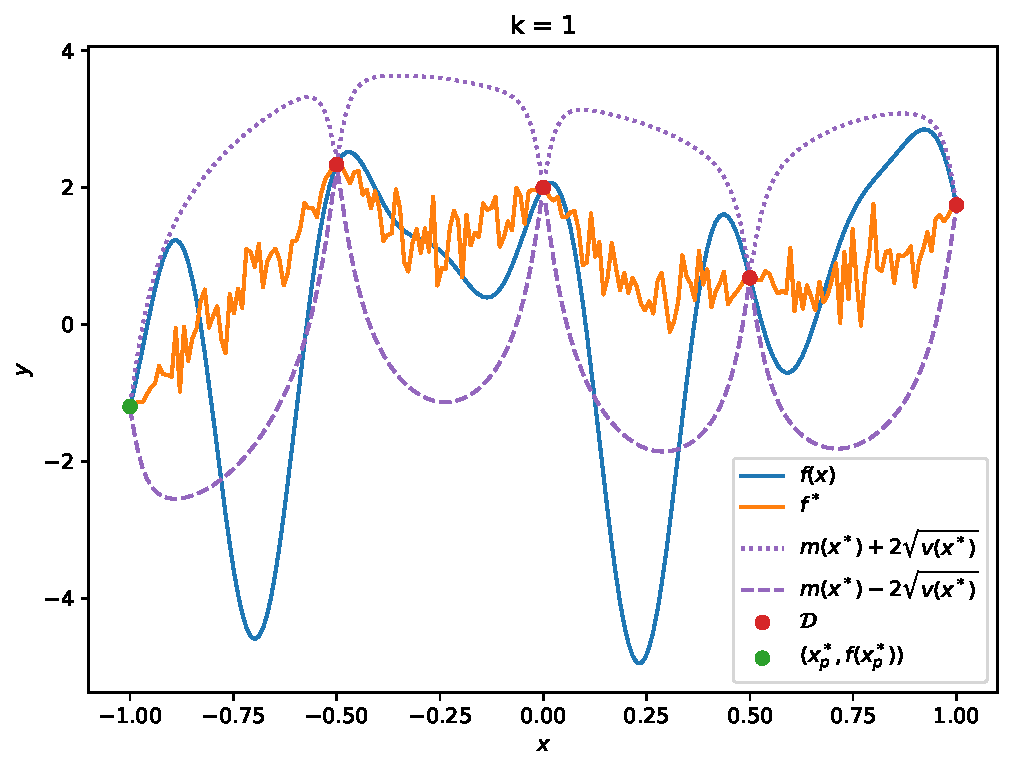
\includegraphics[width=\textwidth]{figures/gp/b2-k_1.pdf}
    \end{subfigure}
    \begin{subfigure}[t]{0.32\textwidth}
        \centering
        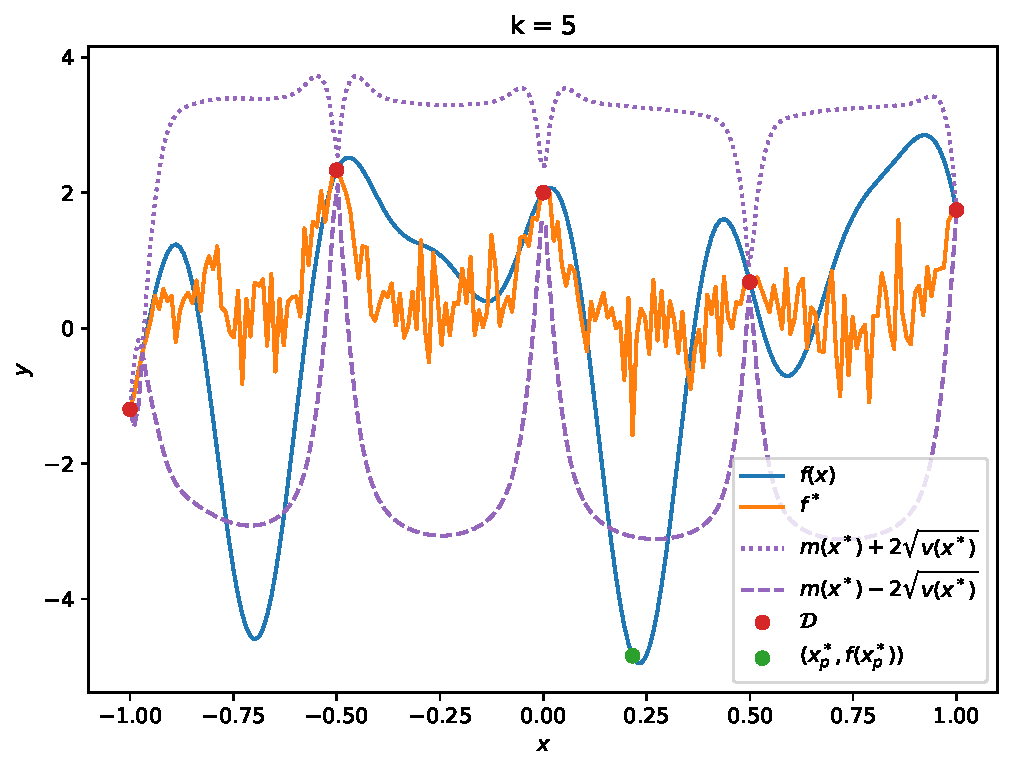
\includegraphics[width=\textwidth]{figures/gp/b2-k_5.pdf}
    \end{subfigure}
    \begin{subfigure}[t]{0.32\textwidth}
        \centering
        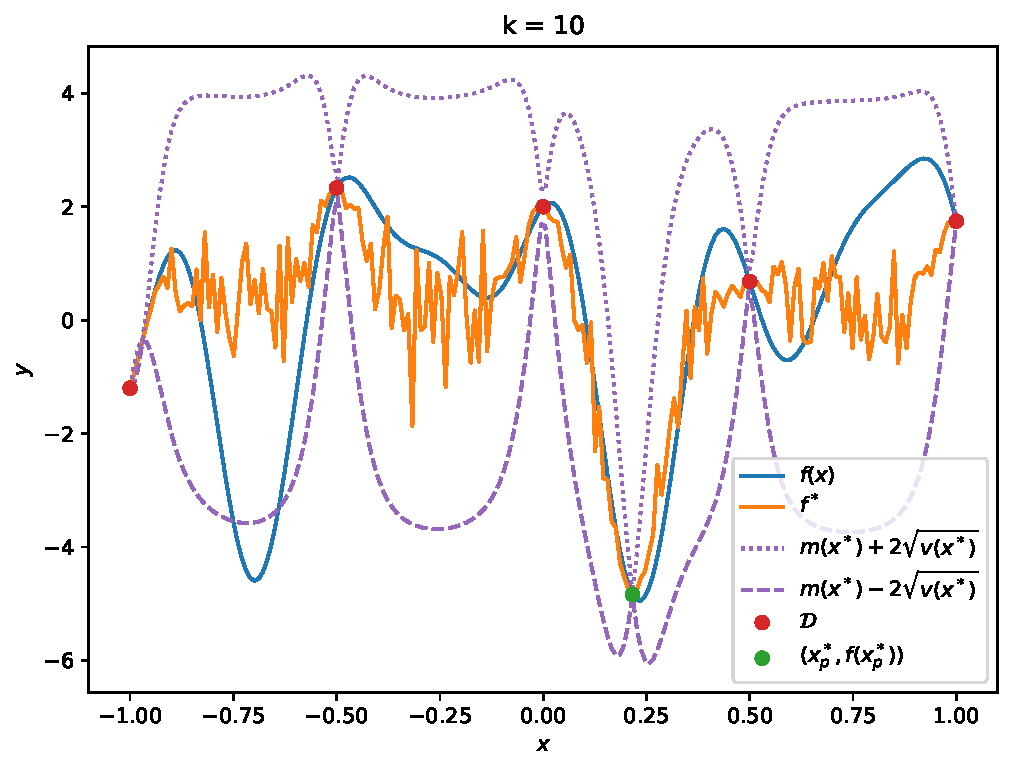
\includegraphics[width=\textwidth]{figures/gp/b2-k_10.pdf}
    \end{subfigure}
    \caption{Plots from running our Bayesian optimization loop at iteration $k$}
    \label{fig:gp:bayesianloop}
\end{figure}